\documentclass[border=2mm]{standalone}
\usepackage{amsmath}
\usepackage{pgfplots}
\usetikzlibrary{3d,calc}

\pgfplotsset{compat=1.12}
\begin{document}

%%%% INCOMING BEAM
 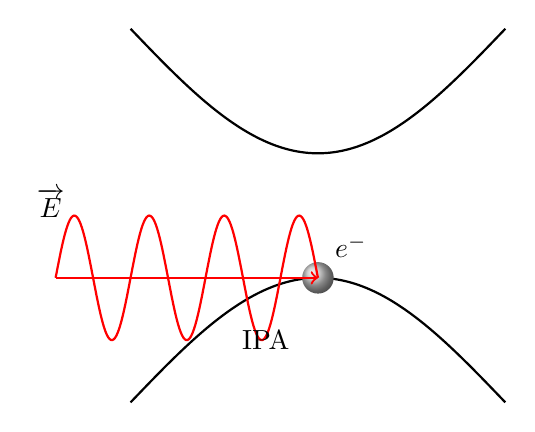
\begin{tikzpicture}
   \begin{axis}[hide axis][
    clip=false,
    xmin=0,xmax=10*pi,
    ymin=-3,ymax=3,
    axis lines=middle,
    xtick=\empty,
    ytick=\empty,
    ]
     \addplot[domain=0:10*pi,samples=200,black,thick]{-1+sin(deg(x/10))}
                               node[right,pos=0.9,font=\footnotesize]{};
     \addplot[domain=0:10*pi,samples=200,black,thick]{2-sin(deg(x/10))}
                               node[right,pos=0.9,font=\footnotesize]{};
     
     \shade[ball color=gray!50!white,opacity=1] (5*pi,0) circle (0.2cm);
     \draw [] (5.2*pi,0.25) node [right] {$e^{-}$};
     
     %%%% INCOMING BEAM FROM -2*pi TO 5*pi -> RANGE OF 7
     \addplot[domain=-2*pi:5*pi,samples=200,red,thick]{0.5*sin(deg(x))}
                               node[right,pos=0.9,font=\footnotesize]{};
     \draw [red, thick, ->] (-2*pi,0) -- (5*pi,0) node [right] {};
     \draw [] (-1.5*pi,0.6) node [left] {$\overrightarrow{E}$};
     \draw [] (4.5*pi,-0.50) node [left] {IPA};
   \end{axis}
 \end{tikzpicture}


% %%%% ELECTRON MOVEMENT
 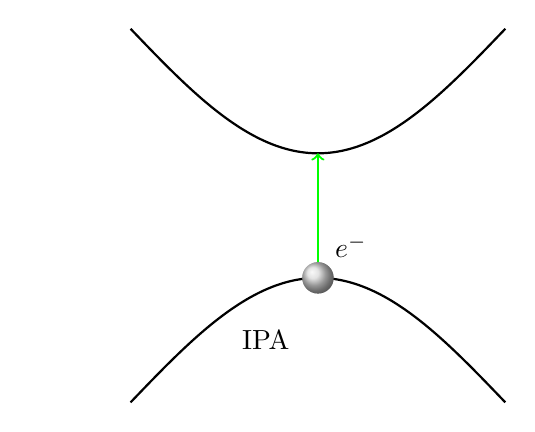
\begin{tikzpicture}
   \begin{axis}[hide axis][
    clip=false,
    xmin=0,xmax=10*pi,
    ymin=-3,ymax=3,
    axis lines=middle,
    xtick=\empty,
    ytick=\empty,
    ]
     %%%% Auxiliar code to have same frame size: objects in white color
     \addplot[domain=-2*pi:1*pi,samples=200,white,thick]{0.5*sin(deg(x))}
                               node[right,pos=0.9,font=\footnotesize]{};
     \draw [white, thick, ->] (-2.03*pi,0) -- (1*pi,0) node [right] {};
     \draw [white] (-1.5*pi,0.6) node [left] {$\overrightarrow{E}$};


     \addplot[domain=0:10*pi,samples=200,black,thick]{-1+sin(deg(x/10))}
                               node[right,pos=0.9,font=\footnotesize]{};
     \addplot[domain=0:10*pi,samples=200,black,thick]{2-sin(deg(x/10))}
                               node[right,pos=0.9,font=\footnotesize]{};

     \draw [green, thick, ->] (5*pi,0) -- (5*pi,1)  node [right] {};
     
     %%%% Electrom moves from (5*pi,0) to (5*pi,1)
     \shade[ball color=gray!50!white,opacity=1] (5*pi,0) circle (0.2cm); %% electron
     \shade[ball color=white!60!white,opacity=0.4] (5*pi,0) circle (0.2cm); %% hole
     \draw [] (5.2*pi,0.25) node [right] {$e^{-}$};
     \draw [] (4.5*pi,-0.50) node [left] {IPA};
   \end{axis}
 \end{tikzpicture}


 
%%% EXCITON
 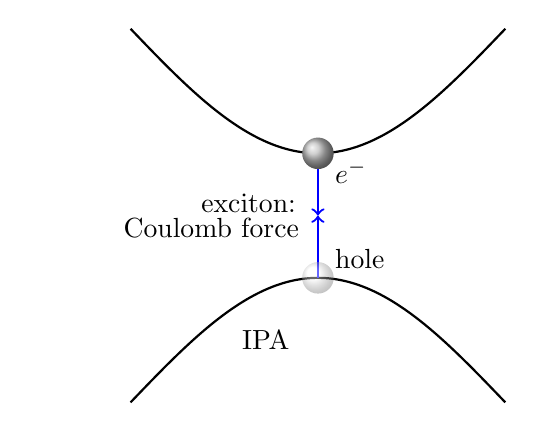
\begin{tikzpicture}
   \begin{axis}[hide axis][
    clip=false,
    xmin=0,xmax=10*pi,
    ymin=-3,ymax=3,
    axis lines=middle,
    xtick=\empty,
    ytick=\empty,
    ]
     %%%% Auxiliar code to have same frame size: objects in white color
     \addplot[domain=-2*pi:1*pi,samples=200,white,thick]{0.5*sin(deg(x))}
                               node[right,pos=0.9,font=\footnotesize]{};
     \draw [white, thick, ->] (-2.03*pi,0) -- (1*pi,0) node [right] {};
     \draw [white] (-1.5*pi,0.6) node [left] {$\overrightarrow{E}$};


     \addplot[domain=0:10*pi,samples=200,black,thick]{-1+sin(deg(x/10))}
                               node[right,pos=0.9,font=\footnotesize]{};
     \addplot[domain=0:10*pi,samples=200,black,thick]{2-sin(deg(x/10))}
                               node[right,pos=0.9,font=\footnotesize]{};

     \draw [blue, thick, ->] (5*pi,1) -- (5*pi,0.5)  node [right] {};
     \draw [blue, thick, ->] (5*pi,0) -- (5*pi,0.5)  node [right] {};
     \draw [] (5*pi,0.6)  node [left] {exciton:  \hspace{3mm}};
     \draw [] (5*pi,0.4)  node [left] {Coulomb force  \hspace{3mm}};
     
     %%%% Electrom moves from (5*pi,0) to (5*pi,1)
     \shade[ball color=gray!50!white,opacity=1] (5*pi,1) circle (0.2cm);
     \draw [] (5.2*pi,0.85) node [right] {$e^{-}$};
     \shade[ball color=white!60!white,opacity=0.4] (5*pi,0) circle (0.2cm);
     \draw [] (5.2*pi,0.15) node [right] {hole};
     \draw [] (4.5*pi,-0.50) node [left] {IPA};
   \end{axis}
 \end{tikzpicture}


\end{document}"
